\documentclass[11pt]{article}

\usepackage{graphicx}
\usepackage{float}
\usepackage{booktabs}
\usepackage{geometry}
\usepackage{caption}
\usepackage{subcaption}
\usepackage{amsmath}

\geometry{a4paper, margin=1in}

\title{Custom FFT Hardware Implementation: \\ Architecture, Verification, and Performance}
\author{EE24BTECH11048\\Nithin K}
\date{}

\begin{document}

\maketitle

\section{Architecture and Implementation}
The custom hardware design implements an 8-point, Radix-2 Fast Fourier Transform (FFT) utilizing a pipelined architecture. The system is split into the core processing module and an automated verification testbench.

\subsection{Pipeline Architecture}
The core processing module (\texttt{fft8\_pipeline}) utilizes a Decimation-In-Time (DIT) algorithm, functioning through the following sequence:
\begin{itemize}
    \item \textbf{Input Buffering and Bit-Reversal:} Serial input samples (\texttt{din\_re}, \texttt{din\_im}) are buffered into a shift register until an 8-point frame is complete. Upon filling, the data is loaded into parallel registers using bit-reversed indexing to prepare for the DIT butterfly stages.
    \item \textbf{Pipelined Butterfly Stages:} The processing is divided into three distinct synchronous stages. Stage 1 executes parallel 2-point butterflies. Stage 2 executes 4-point butterflies. Stage 3 completes the transformation with 8-point butterflies, resolving the final frequency bins. 
    \item \textbf{Fixed-Point Arithmetic:} Twiddle factor multiplications in the final stage are handled by custom fixed-point functions (\texttt{mul\_re} and \texttt{mul\_im}), utilizing arithmetic right shifts to maintain scaling without relying on heavy floating-point logic or vendor DSP blocks. Constants for the twiddle factors are pre-calculated and parameterized.
\end{itemize}

\subsection{Testbench and Verification Logic}
The testbench (\texttt{fft8\_tb}) is designed for automated, self-checking verification. 
\begin{itemize}
    \item \textbf{Stimulus Generation:} A task-based structure is used to clock in five distinct discrete test signals: a cosine tone, an impulse, a DC signal, a complex exponential, and a two-tone combination.
    \item \textbf{Self-Checking Assertions:} Upon assertion of the \texttt{dout\_valid} flag, the testbench automatically checks the magnitude of the 24-bit output bins against the mathematically expected results, outputting a clear PASS/FAIL metric for each test case directly into the simulation console.
\end{itemize}

\section{Functional Verification}
The custom Verilog fixed-point Fast Fourier Transform (FFT) module was verified against a MATLAB floating-point reference model. Various test signals were applied to validate the accuracy of the frequency bins. As shown in the overlay plots, the output of the custom fixed-point implementation aligns with the MATLAB reference across the discrete test cases.

\begin{figure}[H]
    \centering
    \begin{subfigure}[b]{0.48\textwidth}
        \centering
        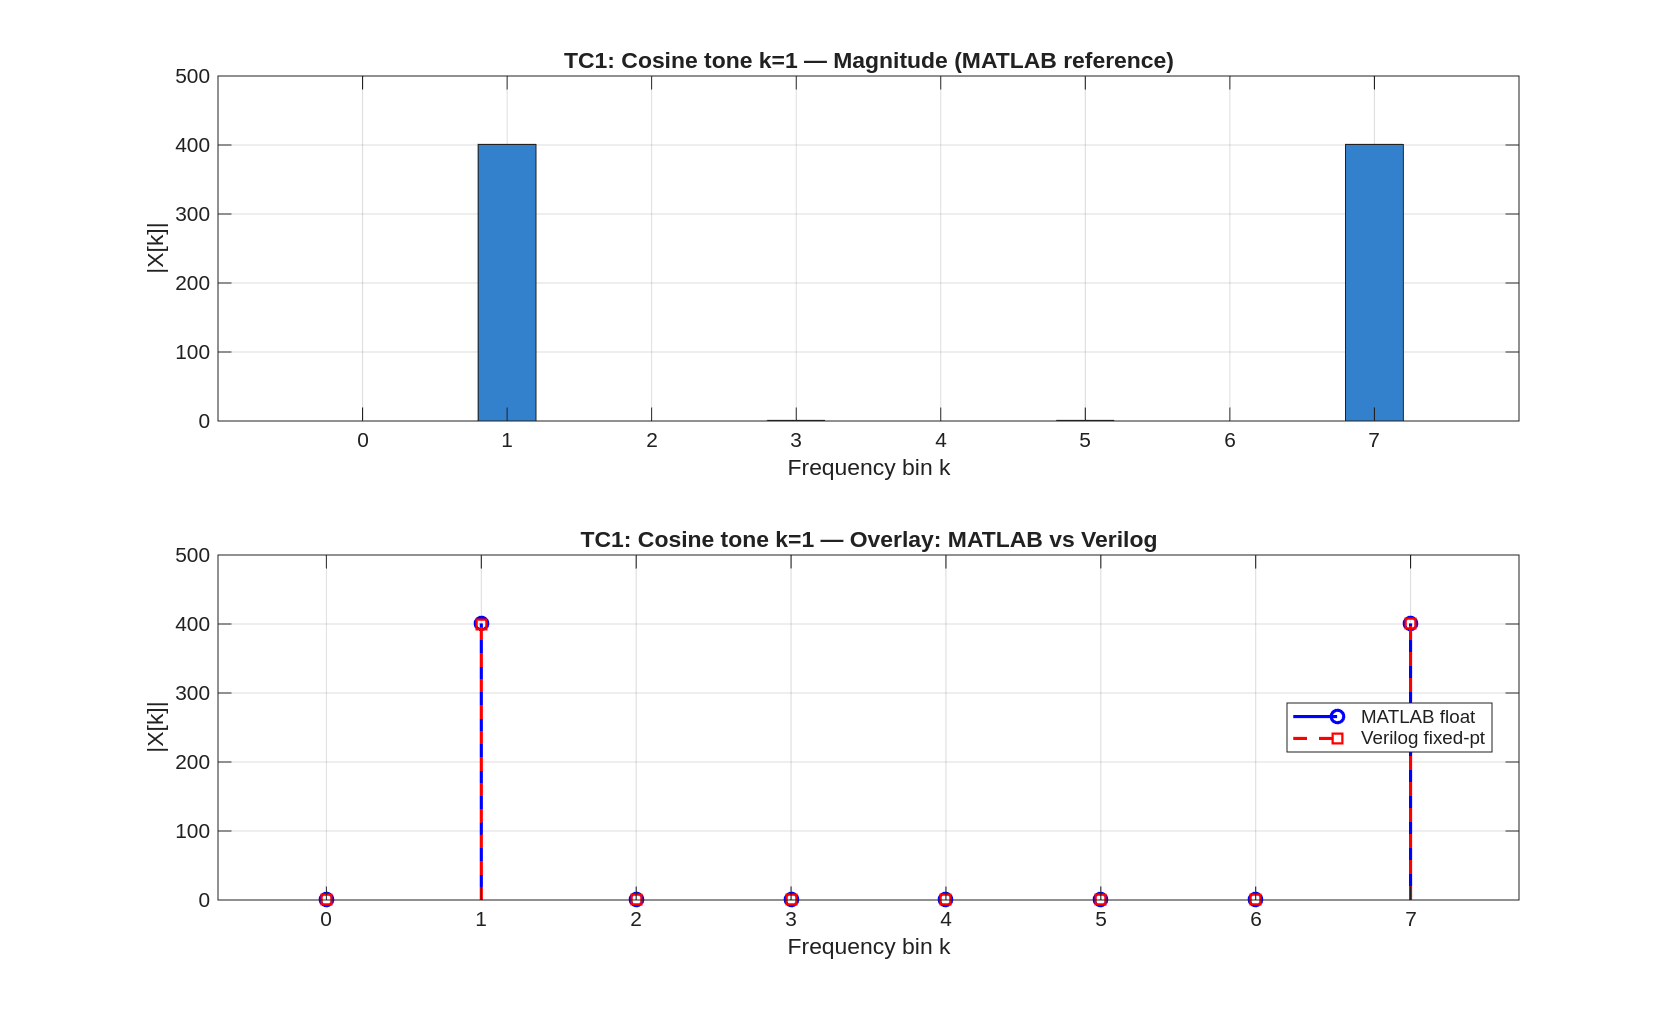
\includegraphics[width=\textwidth]{fft_tc1_spectrum.png}
        \caption{TC1: Cosine tone ($k=1$)}
    \end{subfigure}
    \hfill
    \begin{subfigure}[b]{0.48\textwidth}
        \centering
        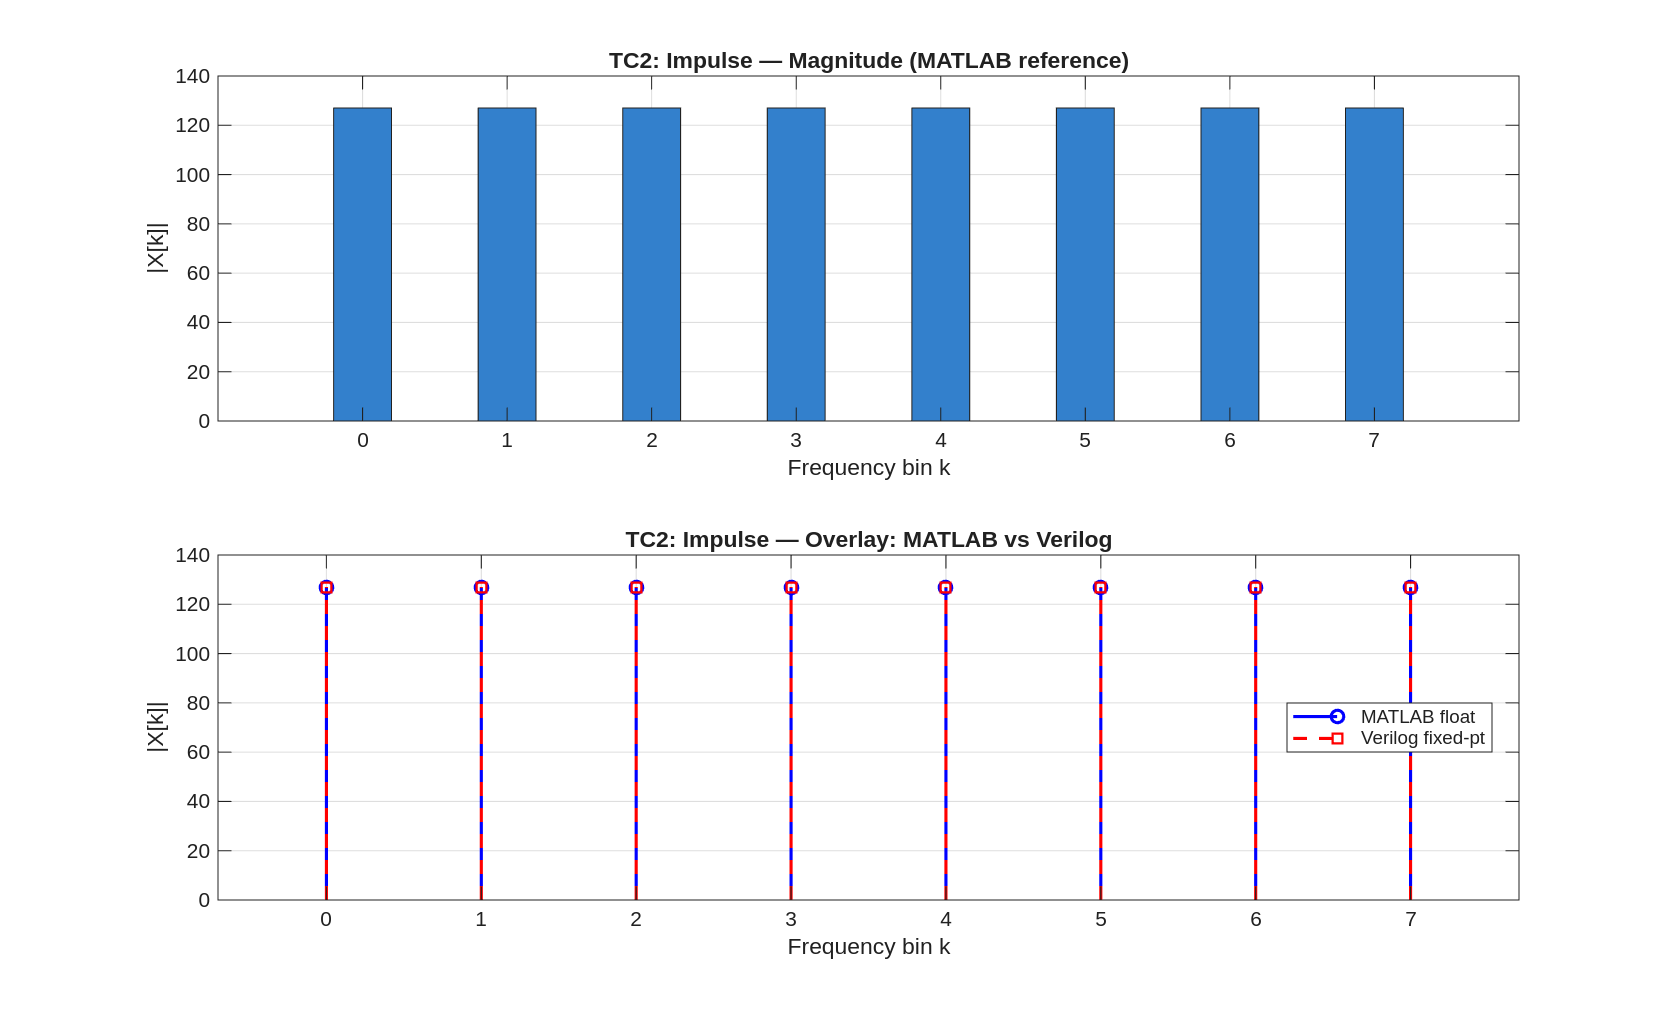
\includegraphics[width=\textwidth]{fft_tc2_spectrum.png}
        \caption{TC2: Impulse}
    \end{subfigure}
    
    \vspace{0.5cm}
    
    \begin{subfigure}[b]{0.48\textwidth}
        \centering
        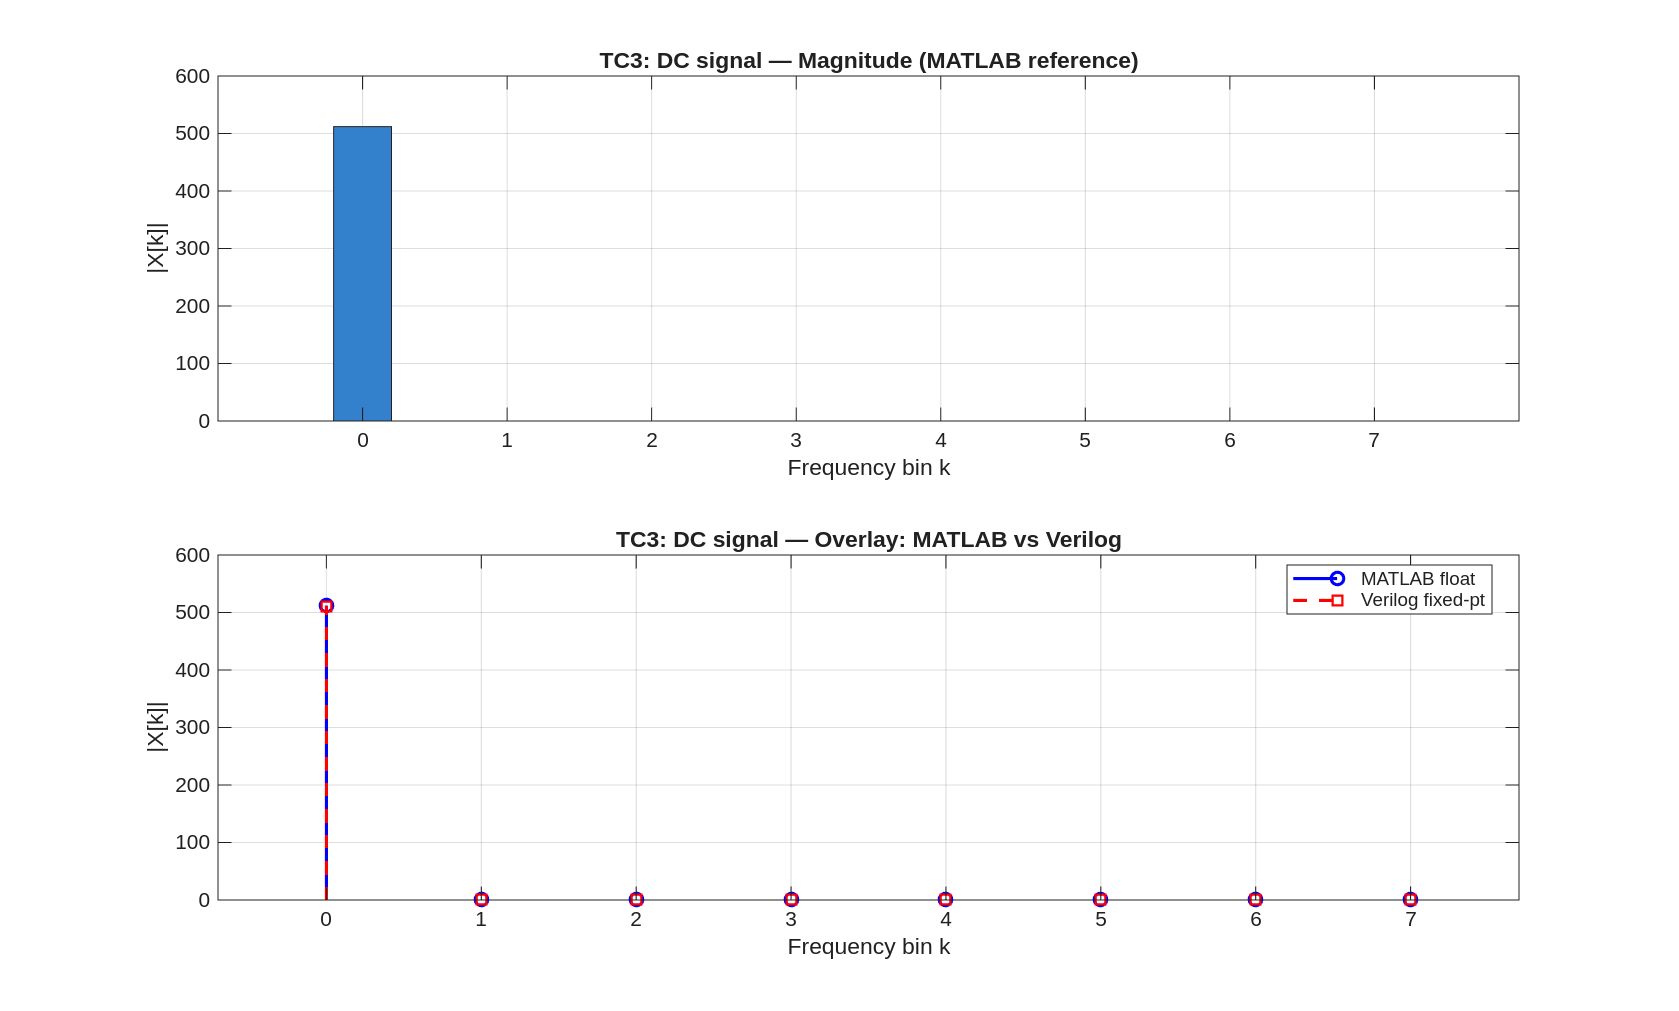
\includegraphics[width=\textwidth]{fft_tc3_spectrum.png}
        \caption{TC3: DC Signal}
    \end{subfigure}
    \hfill
    \begin{subfigure}[b]{0.48\textwidth}
        \centering
        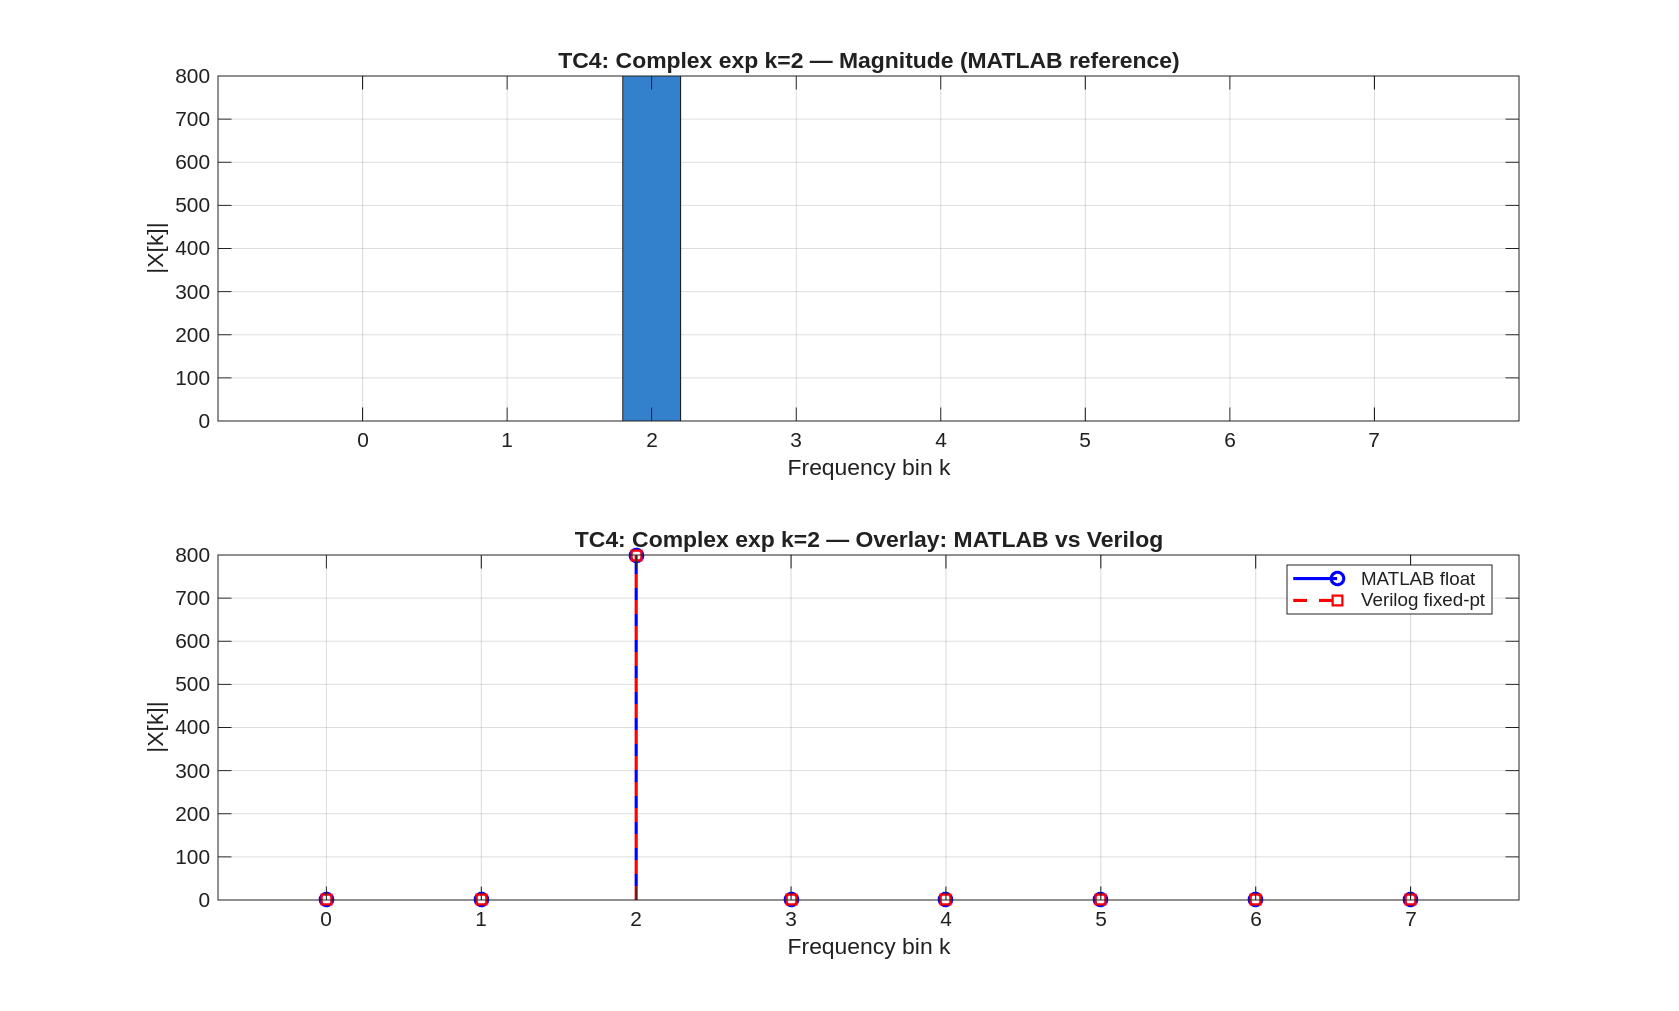
\includegraphics[width=\textwidth]{fft_tc4_spectrum.png}
        \caption{TC4: Complex exponential ($k=2$)}
    \end{subfigure}

    \vspace{0.5cm}

    \begin{subfigure}[b]{0.48\textwidth}
        \centering
        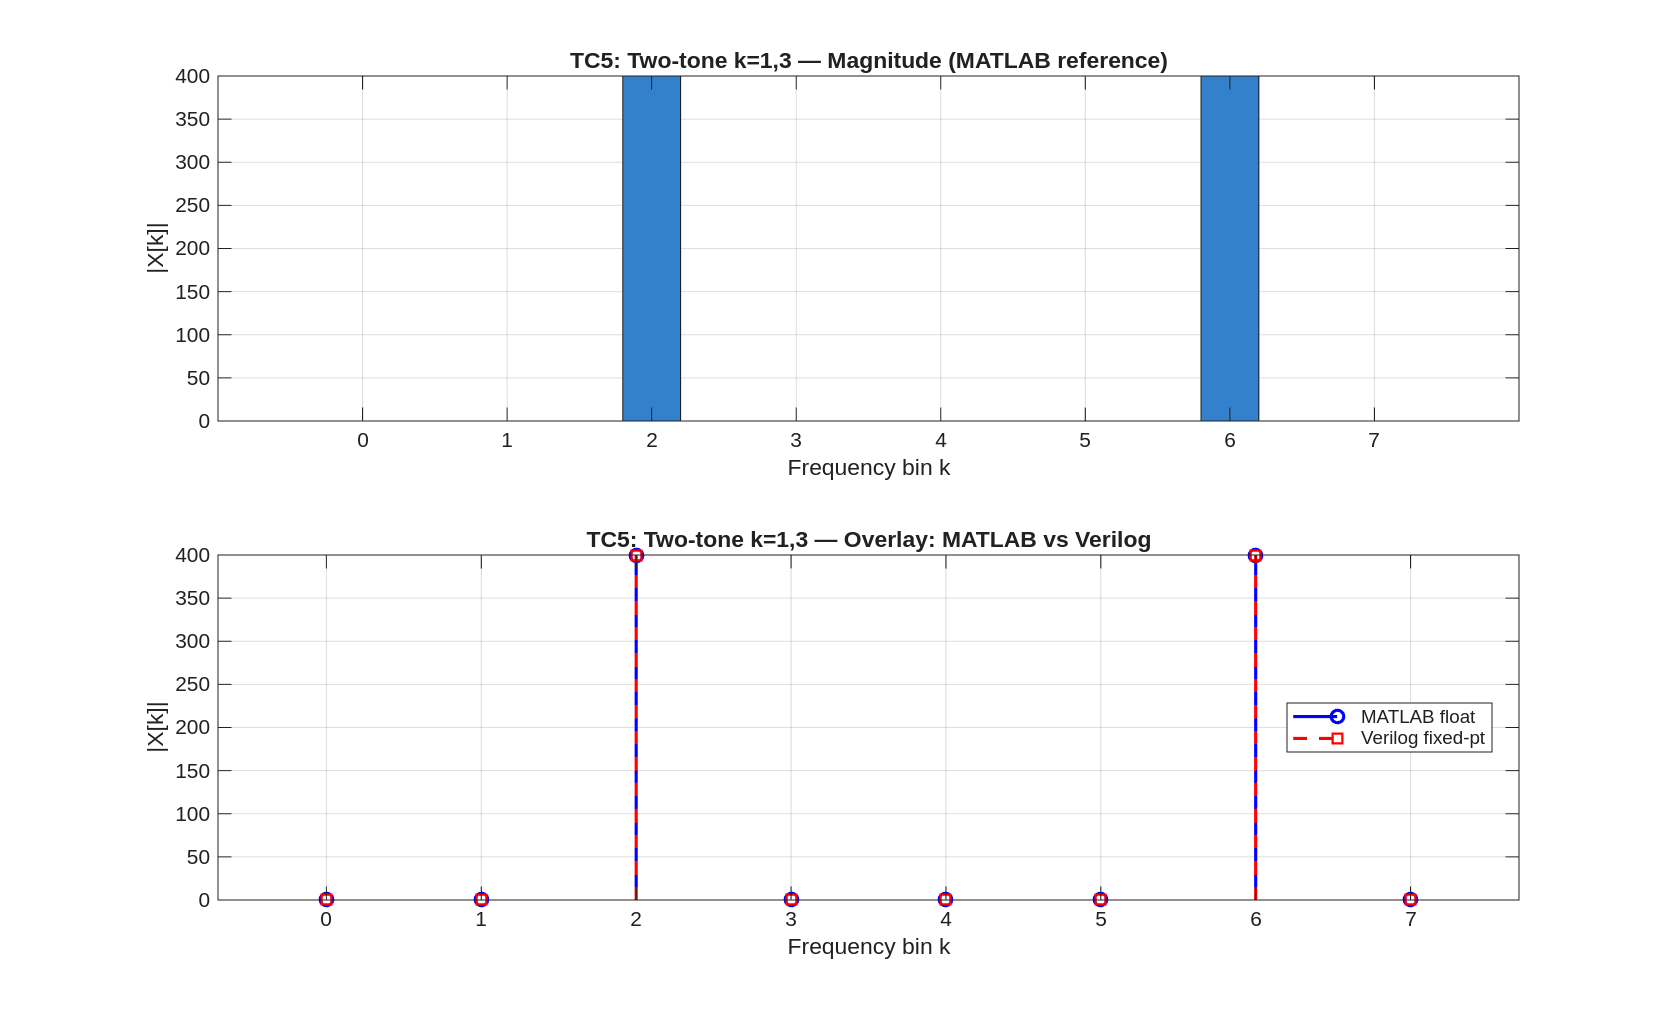
\includegraphics[width=\textwidth]{fft_tc5_spectrum.png}
        \caption{TC5: Two-tone ($k=1, 3$)}
    \end{subfigure}
    \caption{Magnitude spectrum overlays comparing MATLAB floating-point reference vs. Custom Verilog fixed-point implementation.}
    \label{fig:fft_verification}
\end{figure}

\section{Synthesis Results and Performance}
The custom design was synthesized and compared against a standard vendor FFT IP core to document resource utilization and timing metrics. Table \ref{tab:comparison} summarizes the resource allocation and maximum operating frequency ($F_{max}$) extracted from the respective compilation reports. 

\begin{table}[H]
    \centering
    \caption{Performance and Resource Metrics: Custom Verilog vs. Vendor IP}
    \label{tab:comparison}
    \begin{tabular}{@{}lcc@{}}
        \toprule
        \textbf{Metric} & \textbf{Custom Verilog} & \textbf{Vendor IP Core} \\ 
        \midrule
        \textbf{Maximum Frequency ($F_{max}$)} & 238.55 MHz & 168.21 MHz \\
        \textbf{Combinational ALUTs}           & 147        & 761        \\
        \textbf{Dedicated Logic Registers}     & 446        & 1,240      \\
        \textbf{Total Block Memory Bits}       & 0          & 40,960     \\
        \textbf{DSP Blocks}                    & 0          & 2          \\ 
        \bottomrule
    \end{tabular}
\end{table}

\subsection{Throughput Analysis}
Based on the input logic of the custom \texttt{fft8\_pipeline} module, the shift registers require 8 continuous clock cycles to buffer an 8-point data frame. An additional clock cycle is consumed to trigger the \texttt{full} condition and latch the buffered data into the DIT pipeline. This creates a state machine footprint of 9 clock cycles per 8-point data frame.

Using the post-synthesis maximum operating frequency ($F_{max}$) of $238.55\text{ MHz}$, the theoretical maximum throughput for continuous streaming is calculated as follows:

\begin{align*}
    \text{Transform Rate} &= \frac{F_{max}}{9 \text{ cycles/frame}} \approx 26.50 \text{ Mega-transforms/sec} \\
    \text{Sample Throughput} &= 26.50 \text{ MT/s} \times 8 \text{ samples/frame} \approx 212.04 \text{ MSPS}
\end{align*}

This demonstrates that the custom logic path maintains a high-speed data ingestion rate of approximately $212.04\text{ Mega-samples per second}$ while utilizing a minimal logic footprint.

\end{document}
